% !TEX encoding = UTF-8
% !TEX TS-program = pdflatex
% !TEX root = ../tesi.tex
% !TEX spellcheck = it-IT

%**************************************************************
\chapter{Conclusioni}
\label{cap:conclusioni}
Lo scopo principale dello stage era valutare se i prototipi precedentemente realizzati, in collaborazione con un processo d'elaborazione lato \emph{server} che sfruttasse le potenzialità della libreria \emph{PCL}, potessero essere migliorati fino ad ottenere un applicativo, inseribile nel contesto produttivo aziendale, da utilizzare del campo ispettivo. 
I risultati ottenuti sono stati piuttosto soddisfacenti, e quanto realizzato, anche se definito ancora allo stadio prototipale, una volta applicate le necessarie migliorie e raffinamenti, potrà diventare un'applicazione completa di grande utilità nel contesto sopracitato.

%**************************************************************
\section{Prove pratiche di calcolo del volume}
Uno degli obiettivi di primaria importanza del progetto, passo finale del processo di elaborazione e meshing di un Point Cloud, era il calcolo del volume dell'oggetto scansionato, che è uno dei parametri di valutazione del processo ispettivo.
Per rendere l'applicazione utilizzabile nel contesto produttivo è necessario che il calcolo del volume si discosti il meno possibile dal volume reale dell'oggetto. 
Vediamo ora nelle tabelle \ref{tab:calcolo-cestino} e \ref{tab:calcolo-scatola} i risultati ottenuti con l'applicativo nella sua ultima versione, per poi discuterne la bontà ed analizzare meglio il problema.
\subsection{Calcolo del volume di un cestino}
\begin{itemize}
\item \textbf{Oggetto}: Cestino cilindrico
\item \textbf{Volume reale}: 0.5652 $ m^3 $
\end{itemize}
\LTXtable{\textwidth}{tabelle/calcoloVolumeCestino.tex}
\begin{tabular}{l r}
\textbf{Volume medio}: 0.453 $m^3$ & \hspace{115pt} \textbf{Errore medio}: 19.94\% \\
\end{tabular}
\newline

\noindent
I risultati del primo set di test, effettuati scansionando un cestino di forma (approssimativamente) cilindrica non sono particolarmente buoni. L'errore medio del calcolo si assesta infatti attorno al 20\%, con picchi di errore del 42\%. Tali valori sono inaccettabili per un utilizzo produttivo dell'applicativo. La causa principale di tale divergenza è da ricercarsi nella scarsa qualità dei Point Cloud ricostruiti, che soffrivano di evidenti problemi di \emph{drifting}, complice anche la lucidità della superficie metallica del cestino, causa di disturbo al sensore di profondità infrarosso.

\subsection{Calcolo del volume di una scatola}
\begin{itemize}
\item \textbf{Oggetto}: Scatola 
\item \textbf{Volume reale}: 0.42 $ m^3 $
\end{itemize}
\LTXtable{\textwidth}{tabelle/calcoloVolumeScatola.tex}
\noindent
\begin{tabular}{l r}
\textbf{Volume medio}: 0.451 $m^3$ & \hspace{115pt} \textbf{Errore medio}: 14.74\% \\
\end{tabular}
\newline

\noindent
I risultati del secondo set di test, effettuati scansionando una scatola di forma parallelepipoidale, sono molto migliori di quanto osservato nei primi test.
L'errore medio del calcolo si assesta infatti attorno al 14.7\%, anche se la bontà della media è ampiamente sfalsata da un paio di risultati particolarmente erronei, mentre i restanti 8 test riportano un errore inferiore al 10\%.
I Point Cloud ricostruiti della scatola erano molto più accurati di quelli del cestino, di qui i risultati migliori, anche se le ricostruzioni soffrivano ancora parzialmente di problemi di \emph{ghosting} e \emph{drifting}.

\subsection{Conclusioni sul calcolo del volume}
Analizzando i dati raccolti risulta evidente che l'applicazione non è ancora pronta per un uso affidabile sul campo. L'esito del calcolo è strettamente correlato alla qualità della mesh da valutare, quindi dal Point Cloud del quale si effettua il meshing e, risalendo alla radice, alla qualità del Point Cloud inizialmente ricostruito.\\
Per essere utilizzabile in un contesto produttivo l'applicativo deve generare stime il cui errore dev'essere sufficientemente basso (ad es. $\leq$ 5\%), e per ottenere tale risultato è necessario migliorare prima di tutto la ricostruzione iniziale dell'oggetto, come già tentato e discusso nella sezione "\emph{JNI e Point Cloud Registration}" (sez. \ref{sec:registration}).


%**************************************************************
\section{Problemi irrisolti e sviluppi futuri}
Il progetto è nato in tempi molto recenti, dopo circa tre mesi di sviluppo sono stati
prodotti più di un prototipo soddisfacente, l'ultimo dei quali realizzato dal tirocinante. La natura sperimentale del progetto ha fatto emergere durante la realizzazione una serie di problemi spesso non banali, alcuni dei quali irrisolti, ma anche una serie di idee e funzionalità per migliorare l'applicativo. Riporto di seguito alcuni di entrambe le categorie.
\subsection{Problemi irrisolti}
\subsubsection{Artefatti nel Point Cloud}
Durante l'acquisizione dei Point Cloud necessari a ricostruire l'oggetto scansionato, capita spesso che l'acquisizione sia disturbata da alcuni "artefatti", cioè gruppi di punti, tipicamente porzioni di piano, che non hanno corrispettivo nel mondo reale, e degradano la qualità della ricostruzione. Ne vediamo un esempio in figura \ref{fig:artefatti}.
\begin{figure}[!h] 
    \centering 
    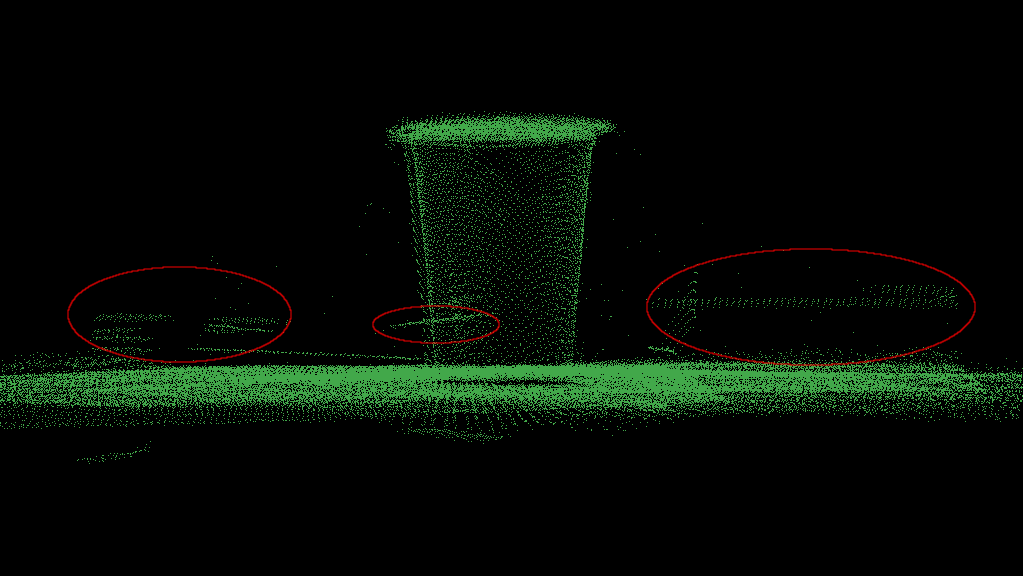
\includegraphics[width=1.0\columnwidth]{varie/artefatti.png} 
    \caption{Esempio di artefatti in un Point Cloud}
   \label{fig:artefatti}
\end{figure}
\newline
L'origine di tali artefatti non è ancora chiara, tra le possibili cause ipotizzate:
\begin{itemize}
\item Un bug nascosto nell'acquisizione dei punti
\item La presenza di riflessi sulle superfici scansionate, che causano problemi al sensore di profondità
\item Problemi di esposizione della fotocamera RGB
\end{itemize}
\noindent
Solitamente gli artefatti possono essere eliminati con successo attraverso il filtraggio \emph{Cluster extraction}, ma capita talvolta che un artefatto vada ad intersecare i punti dell'oggetto scansionato, rendendo così impossibile estrarre una nuvola di punti che rappresenti precisamente l'oggetto.

\subsubsection{Surriscaldamento e consumo della batteria}
Il \emph{device Tango} è sottoposto ad un notevole sforzo computazionale durante l'acquisizione dei Point Cloud, a causa dell'utilizzo di più sensori e di pesanti elaborazioni parallele, ed è facilmente predisposto al surriscaldamento (che ne peggiora le prestazioni) e ad un consumo eccessivo della batteria. Non era negli scopi dello stage affrontare tali problematiche, ma in un futuro potrebbe essere necessario risolverle rendendo più performante il processo di aquisizione.

\subsubsection{Limiti del device}
Durante l'acquisizione dei Point Cloud sono emersi alcuni problemi dovuti ai limiti fisici del \emph{device Tango}, dovuti in particolare all'utilizzo dei sensori di profondità a luce infrarossa, che non funzionano (quindi non è possible acquisire dei punti) nei seguenti casi:
\begin{itemize}
\item Superfici riflettenti o molto lucide.
\item Superfici di colore molto scuro, tendente al nero
\end{itemize}
In questi casi il segnale infrarosso viene completamente assorbito o deviato, e non si ottiene quindi nessun feedback. Possiamo vedere gli effetti di tale problema in figura \ref{fig:nero}, in cui si nota come alle parti metalliche della sedia corrisponda l'assenza di punti.
\begin{figure}[!h] 
    \centering 
    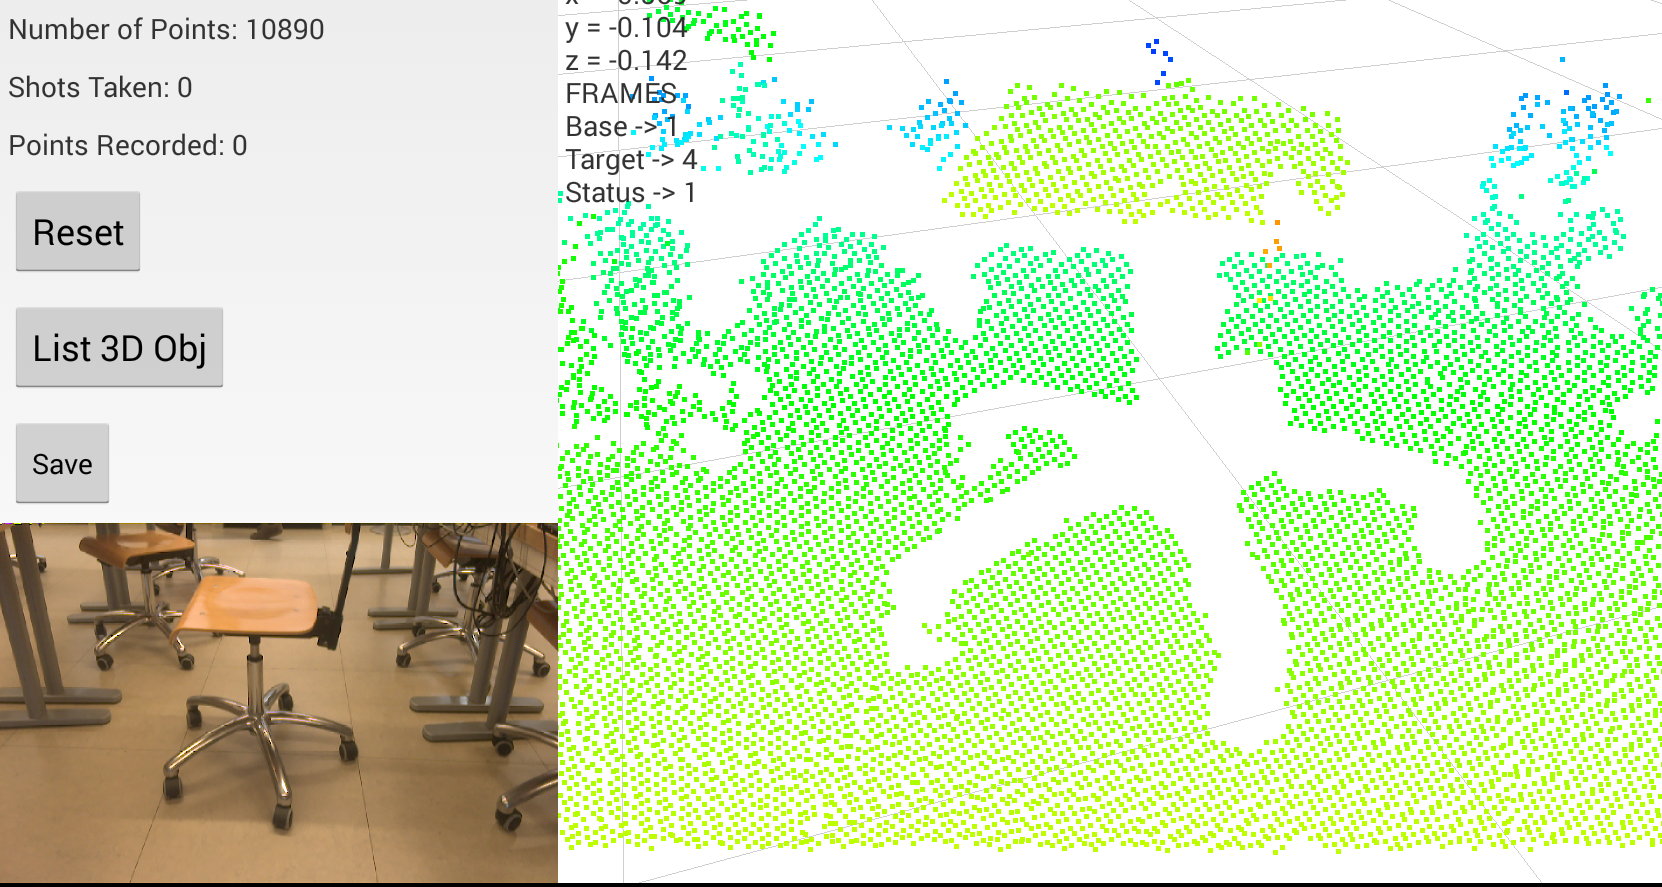
\includegraphics[width=1.0\columnwidth]{varie/nero.png} 
    \caption{Esempio di problemi nell'acquisizione di superfici lucide}
   \label{fig:nero}
\end{figure}
\newline
Non potendo ovviamente agire sulle capacità hardware del dispositivo, l'unica strada possibile per arginare il problema è di implementare un sistema software capace di ricostruire i punti mancanti, compito che esula dagli scopi dello stage.

\subsection{Sviluppi futuri}
\subsubsection{Point Cloud Registration}
Come già citato nelle sezioni \ref{sec:registration} e \ref{sec:volume}, la \emph{Registration} tramite algoritmo ICP di Point Cloud è una funzionalità indispensabile a migliorare la precisione del calcolo del volume, e quindi allo sviluppo futuro dell'applicazione. \\
Vi sono due strade percorribili per attuare tale miglioria:
\begin{itemize}
\item \textbf{ICP su \emph{tablet}}: opzione preferita, la cui attuazione con GOICP non ha dato i risultati sperati, ma che vale la pena esplorare ulteriormente, testando altri algoritmi ICP, adattando GOICP o implementando un algoritmo ICP ad hoc in Java. Resta da valutare attentamente però l'effettiva capacità del \emph{tablet} di eseguire in tempi accettabili le computazioni richieste
\item \textbf{ICP lato server}: la libreria \emph{PCL} offre anche un algoritmo ICP, che è stato testato con successo, ma che non è stato possibile importare su \emph{tablet} a causa della complessità dello stesso. Per effettuare ICP su \emph{server} è quindi necessario che il \emph{client} invii non più il Point Cloud ricostruito, ma le singole scansioni una ad una. Tale approccio non è praticabile nel contesto d'uso nel quale dovrà inserirsi l'applicativo, che non prevede una connessione internet stabile, mancanza che renderebbe inaccettabilmente lungo l'intero processo di acquisizione ed elaborazione.
\end{itemize}
\noindent
L'implementazione di ICP su \emph{tablet} sembra quindi essere l'alternativa migliore, e senza dubbio è una funzionalità che migliorerebbe significativamente le potenzialità dell'applicativo.

\subsubsection{Comparazione con modello 3D esatto}
Una funzionalità di indubbia utilità nel campo ispettivo sarebbe la possibilità di confrontare le mesh generate con modelli tridimensionali esatti degli oggetti scansionati, in modo da valutarne la conformità ed evidenziarne eventualì deformità e difetti.\\
 Si pensi ad esempio all'utilizzo in una catena di montaggio per valutare la conformità dei beni prodotti con i modelli di partenza, o al controllo dei danni per beni che siano stati sottoposti a trasporto.
L'implementazione di tale funzionalità richiederà prima di tutto una maggiore precisione delle mesh generate, che dovranno anche essere completamente "chiuse", dato che al momento le mesh mancano della parte inferiore, che dev'essere adeguatamente ricostruita.

%\subsubsection{Miglioramento server}

\subsubsection{Integrazione con l'applicazione VIC}
L'azienda fornisce ai suoi dipendenti un'applicazione che permette di automatizzare le mansioni ispettive, con l'inserimento nel database aziendale di ogni nuova ispezione o \emph{job}, permettendo all'utente di compilare diversi \emph{form} per definirne scopi e risultati, per fornire così in tempo reale un rapporto dettagliato e standardizzato del lavoro svolto. In questo ambito un integrazione con i risultati ottenuti tramite i \emph{device Tango} potrebbe quindi fornire \emph{report} più dettagliati e velocizzare le operazioni d'ispezione.

\subsubsection{Meshing con textures}
Il prodotto fornisce delle buone ricostruzioni tridimensionali per quanto riguarda la forma e le dimensioni dell'oggetto; ai fini ispettivi del contesto aziendale, di fatto, non c'è bisogno d'altro. Ciononostante le ricostruzioni visualizzate su \emph{tablet}, essendo formate da soli triangoli privi di textures, sono spesso di difficile comprensione da parte dell'utenza.\\ Un primo passo per migliorare tale visualizzazione è stato di permettere l'applicazione di textures standard alla mesh, che perlomeno aiutano a definire meglio la volumetria dell'oggetto. Il passo successivo da implementare per rendere più immediato il riconoscimento dell'oggetto da parte dell'utente sarà di poter applicare textures liberamente scelte, o meglio ancora, di applicare texture che corrispondano ai colori e materiali dell'oggetto scansionato.
Questo sviluppo, oltre a migliorare grandemente l'aspetto grafico del sistema, lo renderebbe anche più vendibile.\\

%**************************************************************
\section{Consuntivo finale}
Il periodo di stage ha avuto inizio il 12 Luglio 2016 ed è terminato l'8 Settembre 2016, per una durata totale di 320 ore.
Seguono in tabella \ref{tab:preventivo-consuntivo} le ore preventivate per le attività dello satge, confrontate con le ore realmente impiegate.
\begin{table}[h]
	\begin{center}
	  \begin{tabular}{| l | c | c | c | c |}
	    \hline
	    \textbf{Attività} & \textbf{Preventivo} & \textbf{Consuntivo} & \textbf{Diff} & \textbf{Diff \%} \\ \hline
	    Studio preliminare & 40 & 50 & +10 & + 25\%\\
	    \hline
	    Analisi dei requisiti e progettazione & 40 & 55 & +15 & +37.5\%\\
	    \hline
	    Calcolo del poligono e del volume & 120 & 85 & - 35 & - 29\%\\
	    \hline
	    Sviluppo dell'applicazione & 80 & 85 & +5 &  + 6\%\\
	    \hline
	    Testing e valutazione dei risultati & 40 & 45 & +5 & +12.5\%\\
	    \hline

	    Totale & 320 & 320 & +0 & +0\%\\
	    \hline
	  \end{tabular}
	\end{center}
	\caption{Distribuzione ore preventivo e consuntivo}
	\label{tab:preventivo-consuntivo}
\end{table}
\newline
Lo ore totali sono state rispettate senza subire variazioni.\\
La ripartizione interna invece ha subito variazioni consistenti nelle prime fasi del progetto, quali lo studio preliminare e l'analisi dei requisiti, le cui ore sono state sottostimate. L'esplorazione intensiva della documentazione \emph{PCL} si è rivelata invece più dispendiosa di quanto calcolato, ed ah portato ad un maggior numero di ore rivolto all'estensione dello studio di fattibilità e dei requisiti utente.\\
 L'accurato studio iniziale ha però permesso di svolgere con profitto e in tempi minori l'attività di "Calcolo del poligono e del volume", le cui ore preventivate sono state largamente sovrastimate. Le risorse risparmiate in quest'ultima fase sono state però ripartite parzialmente nelle fasi successive, ed hanno permesso di effettuare valutazioni più numerose ed accurate durante la fase di testing.


\newpage
%**************************************************************
\section{Raggiungimento degli obiettivi}
Gli obbiettivi riportati inizialmente nel piano di lavoro erano i seguenti:
\begin{itemize}
	\item \textbf{Obbligatori}
	\begin{itemize}
		\item \underline{\textit{ob01}}: studio dello stato attuale del progetto;
		\item \underline{\textit{ob02}}: ideazione di una soluzione per il calcolo del poligono rappresentante un oggetto e per il calcolo del relativo volume;
		\item \underline{\textit{ob03}}: implementazione prototipo in grado di calcolare un poligono rappresentante un oggetto e il relativo volume;
		\item \underline{\textit{ob04}}: implementazione app come indicato nella sezione "Struttura applicazione" del documento "Relazione app per Project Tango" fornito dall’azienda;
		\item \underline{\textit{ob05}}: Testing dell’applicazione e valutazione della precisione dei risultati ottenuti.
	\end{itemize}
	
	\item \textbf{Desiderabili}
	\begin{itemize}
		\item \underline{\textit{de01}}: perfezionare calcolo del poligono (cavità nell’oggetto, eliminazione dati di sfondo/rumore);
		\item \underline{\textit{de02}}: perfezionare calcolo del volume (cavità nell’oggetto);
	\end{itemize}
	
	\item \textbf{Opzionali}
	\begin{itemize}
		\item \underline{\textit{op01}}: ottimizzazione della comunicazione con il \emph{server} nel caso risultasse necessaria.
	\end{itemize} 
\end{itemize}
\noindent 
Gli obbiettivi obbligatori definiti sono stati tutti pienamente raggiunti.
Per quanto riguarda gli obbiettivi desiderabili invece:
\begin{itemize}
	\item \underline{\textit{de01}}: \'E stato parzialmente soddisfatto, con l'eliminazione degli elementi di disturbo dal Point Cloud. Non è stata implementata invece una tecnica efficiente per il calcolo delle cavità del poligono.
	\item \underline{\textit{de02}}: Non raggiunto
\end{itemize}
\noindent
L'obbiettivo opzionale \underline{\textit{op1}} è stato raggiunto con l'implementazione di meccanismi di fallback lato \emph{client} in caso di mancata connessione.

\subsection{Requisiti}
Dagli obiettivi posti nel piano di lavoro e dai casi d'uso prodotti sono stati ricavati i requisiti esposti nel capitolo \ref{cap:analisi-requisiti}. Seguono le tabelle (\ref{tab:esito-requisiti-funzionali}, \ref{tab:esito-requisiti-qualitativi}, \ref{tab:esito-requisiti-vincolo}, \ref{tab:esito-requisiti-prestazionali}) di soddisfacimento di questi ultimi divisi per categorie.

\newpage
\subsubsection{Requisiti Funzionali}
\LTXtable{\textwidth}{tabelle/esitoFunzionali.tex}

\newpage
\subsubsection{Requisiti Qualitativi}
\LTXtable{\textwidth}{tabelle/esitoQualitativi.tex}

\subsubsection{Requisiti di Vincolo}
\LTXtable{\textwidth}{tabelle/esitoVincolo.tex}

\subsubsection{Requisiti Prestazionali}
\LTXtable{\textwidth}{tabelle/esitoPrestazionali.tex}

\subsubsection{Esito finale}
In tabella \ref{tab:esito-requisiti-finale} possiamo vedere i dati riassuntivi del soddisfacimento di tutti i requisiti.
\begin{longtable}{l c c c}  
\endhead
\hline\hline
\multicolumn{4}{c}{\textbf{Requisiti funzionali}}\\
\hline
\textbf{Tipologia} & \textbf{Totali} & \textbf{Soddisfatti} & \textbf{Percentuale}\\
Obbligatori 		&		27		&			27			&		100\%			\\
Desiderabili 		&		9		&			9			&		100\%			\\
Opzionali			&		2		&			0			&		0\%			\\
\hline\hline
\multicolumn{4}{c}{\textbf{Requisiti qualitativi}}\\
\hline
\textbf{Tipologia} & \textbf{Totali} & \textbf{Soddisfatti} & \textbf{Percentuale}\\
Obbligatori 		&		2		&			2			&		100\%			\\
Desiderabili 		&		1		&			0			&		0\%				\\
\hline\hline
\multicolumn{4}{c}{\textbf{Requisiti di vincolo}}\\
\hline
\textbf{Tipologia} & \textbf{Totali} & \textbf{Soddisfatti} & \textbf{Percentuale}\\
Obbligatori 		&		3		&			3			&			100\%		\\
\hline\hline
\multicolumn{4}{c}{\textbf{Requisiti prestazionali}}\\
\hline
\textbf{Tipologia} & \textbf{Totali} & \textbf{Soddisfatti} & \textbf{Percentuale}\\
Obbligatori 		&		2		&			2			&			100\%		\\
Desiderabili 		&		7		&			6			&			85\%		\\
\hline\hline
\multicolumn{4}{c}{\textbf{Totale}}\\
\hline
\textbf{Tipologia} & \textbf{Totali} & \textbf{Soddisfatti} & \textbf{Percentuale}\\
Obbligatori 		&		34		&			34			&		100\%			\\
Desiderabili 		&		17		&			15			&		89\%			\\
Opzionali			&		2		&			0			&		0\%			\\


\hline
\caption{Soddisfacimento totale dei requisti}
\label{tab:esito-requisiti-finale}
\end{longtable}

%**************************************************************
\section{Conoscenze acquisite}
Dal punto di vista formativo l'attività di \emph{stage} è stata estremamente positiva. Ha arricchito il mio bagaglio personale di competenze professionali non banali.\\

\noindent
La richiesta di applicazioni in ambito \emph{mobile} è in continuo aumento negli ultimi anni. Per questo l'apprendimento della progettazione e sviluppo delle applicazioni mobili \emph{Android} è certamente una conscenza preziosa ed immancabile per un inserimento nel mondo dell \emph{IT}.\\
\noindent
L'approccio ad una tecnologia sperimentale ed ancora di nicchia come \emph{Project Tango} è un notevole vantaggio in ambito occupazionale in quanto gli sviluppatori nell'ambito sono ancora scarsi. Inoltre il rilascio del primo \emph{smartphone} commerciale dotato dei sensori \emph{Tango} è stato annunciato da un noto marchio per l'autunno 2016; se dovesse prendere campo anche in ambito \emph{customer} ci sarebbe certamente una grande richiesta di sviluppatori con esperienza vista la scarsità di applicazioni capaci di sfruttare le potenzialità che questo tipo di \emph{device} ha da offrire.\\
\noindent
In ambito aziendale si è usato \emph{Java} come linguaggio di programmazione ed \emph{Android Studio} come \emph{IDE}. La curva di apprendimento di questi strumenti è stata piuttosto rapida grazie all'esperienza già maturata in ambito accademico con \emph{Java} ed \emph{IntelliJ}, su cui è basato \emph{Android Studio}. Più complessa si è rivelata l'assimilazione e la comprensione del \emph{Framework Jni}, sia a causa della sua intrinseca complessità sia al fatto che \emph{Android Studio} lo supporta solo in \emph{release} sperimentale. Il suo utilizzo nello stage è stato possibile solo nell'ultima settimana, grazie al miglior supporto del framework introdotto nelle ultime versioni sperimentali di \emph{Android Studio}. In ogni caso molte applicazioni \emph{mobile}, specialmente in ambito grafico, ne fanno uso, quindi ai fini del curriculum si è rivelata comunque un'esperienza fruttuosa.\\
\noindent
L'apprendimento delle potenzialità della libreria \emph{PCL} e la gestione dei \emph{Point Cloud} è un'altra competenza non banale, che può dare i suoi frutti in molti campi della \emph{Computer grafica}. Lo studio di \emph{PCL} è stata inoltre un'occasione formativa importante, dalla quale ho imparato ad approcciare in autonomia una libreria vasta e complicata, ed estrapolarne le funzionalità richieste, le metodologie d'utilizzo e le \emph{best practices}.\\

\noindent
Il tirocinio è stato quindi un'esperienza formativa interessante e stimolante, dalla quale esco profondamente arricchito nelle conoscenze e nelle capacità produttive.
